\documentclass[10pt,twocolumn,letterpaper]{article}

\usepackage{dependable_dnn}
\usepackage{times}
\usepackage{epsfig}
\usepackage{graphicx}
\usepackage{amsmath}
\usepackage{amssymb}
\usepackage{subfigure}
\usepackage[table, dvipsnames]{xcolor}

% Include other packages here, before hyperref.

% If you comment hyperref and then uncomment it, you should delete
% egpaper.aux before re-running latex.  (Or just hit 'q' on the first latex
% run, let it finish, and you should be clear).
\usepackage[pagebackref=true,breaklinks=true,letterpaper=true,colorlinks,bookmarks=false]{hyperref}

\iccvfinalcopy % *** Uncomment this line for the final submission

\def\iccvPaperID{} % *** Enter the Paper ID here
\def\httilde{\mbox{\tt\raisebox{-.5ex}{\symbol{126}}}}

% Pages are numbered in submission mode, and unnumbered in camera-ready
\ificcvfinal\pagestyle{empty}\fi

\begin{document}

%%%%%%%%% TITLE - PLEASE UPDATE
\title{Transformer Meets Tracker: \\Exploiting Temporal Context for Robust Visual Tracking
\\ {\rm {\normalsize Seungmin Lee (profile2697@gmail.com; 2020-20866), \\Dept. of Electrical and Computer Engineering, Seoul National University}}}   % **** Enter the paper title and student information here

\maketitle
\thispagestyle{empty}

\section{Introduction and Motivation}
To successfully tracking objects in videos, we need to capture valuable temporal information existing across frames. Unfortunately, most existing methods are based on per-frame detection, limiting the ability to model temporal relationships between frames. Moreover, those methods assume that tracking targets move smoothly while targets in real-world videos move noisily and are blurred or occluded.  This paper claims that a siamese-like tracking pipeline combined with a transformer can effectively mitigate the problems by modeling temporal relationships.

\begin{figure}[b]
	\centering
	\subfigure[The Proposed Siamese-like Pipeline]{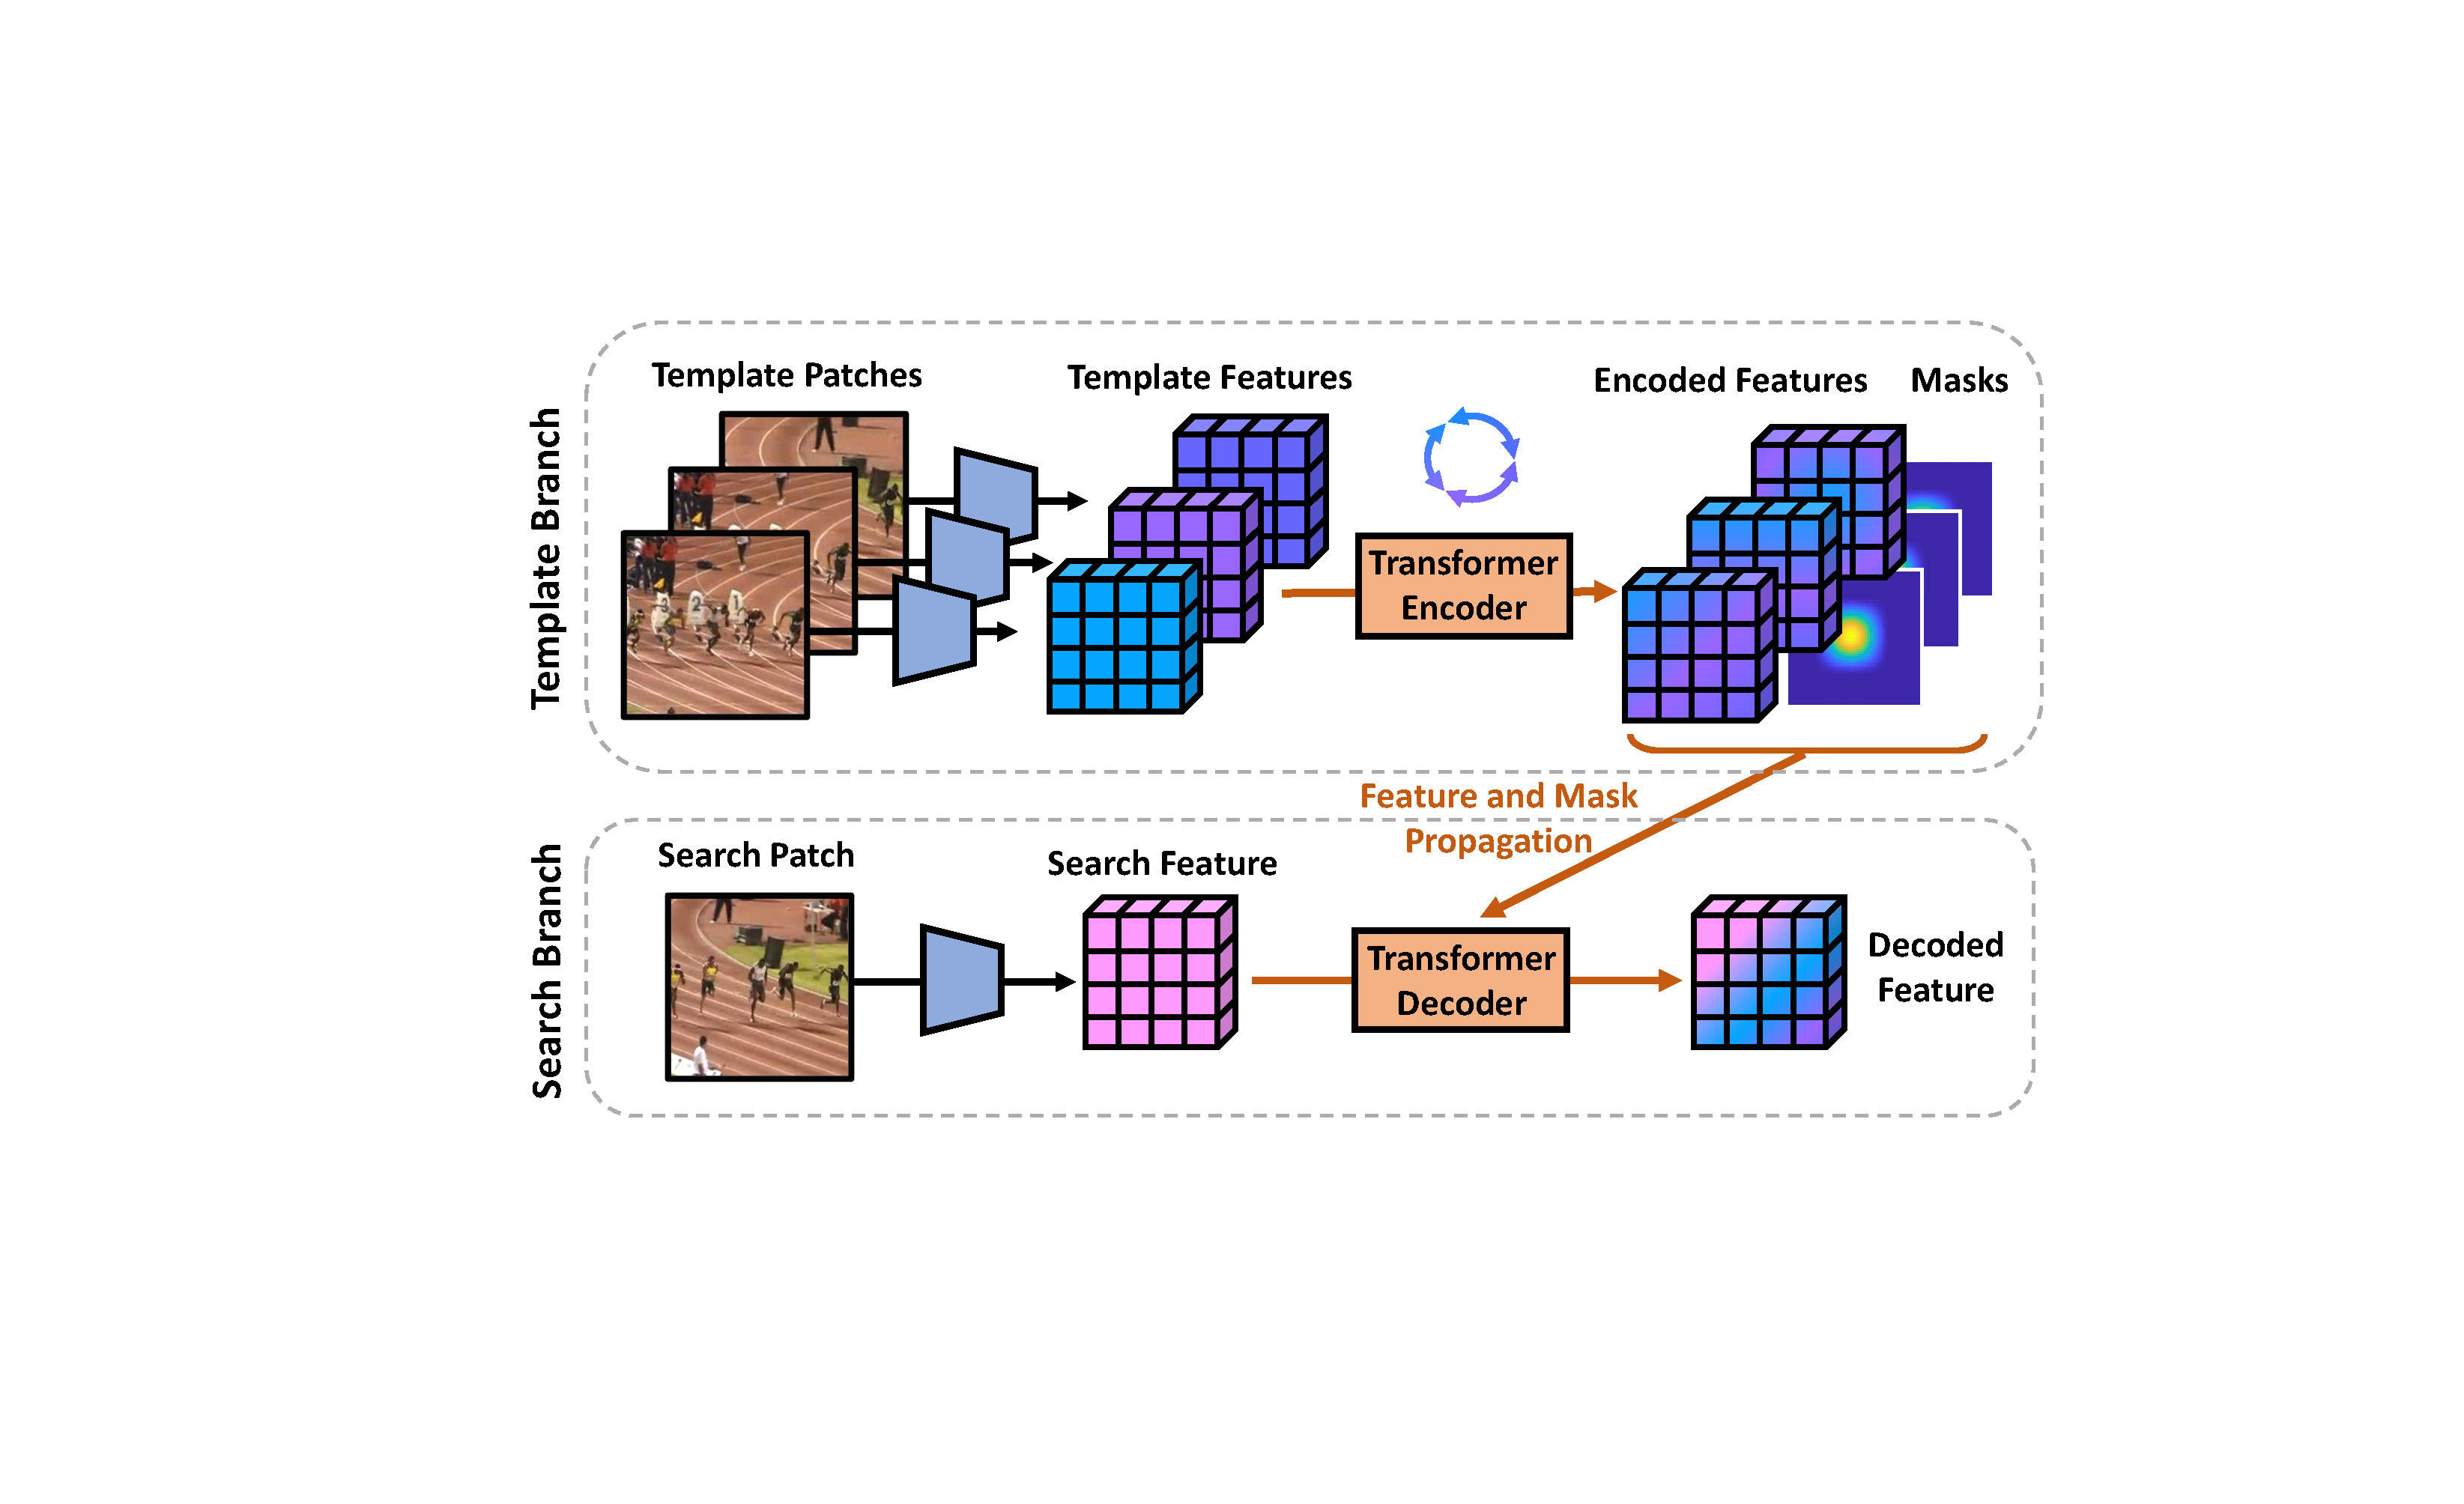
\includegraphics[width=4cm, height=3cm]{assets/2.pdf}}
	\subfigure[The Encoder-Decoder Transformer used in the branches]{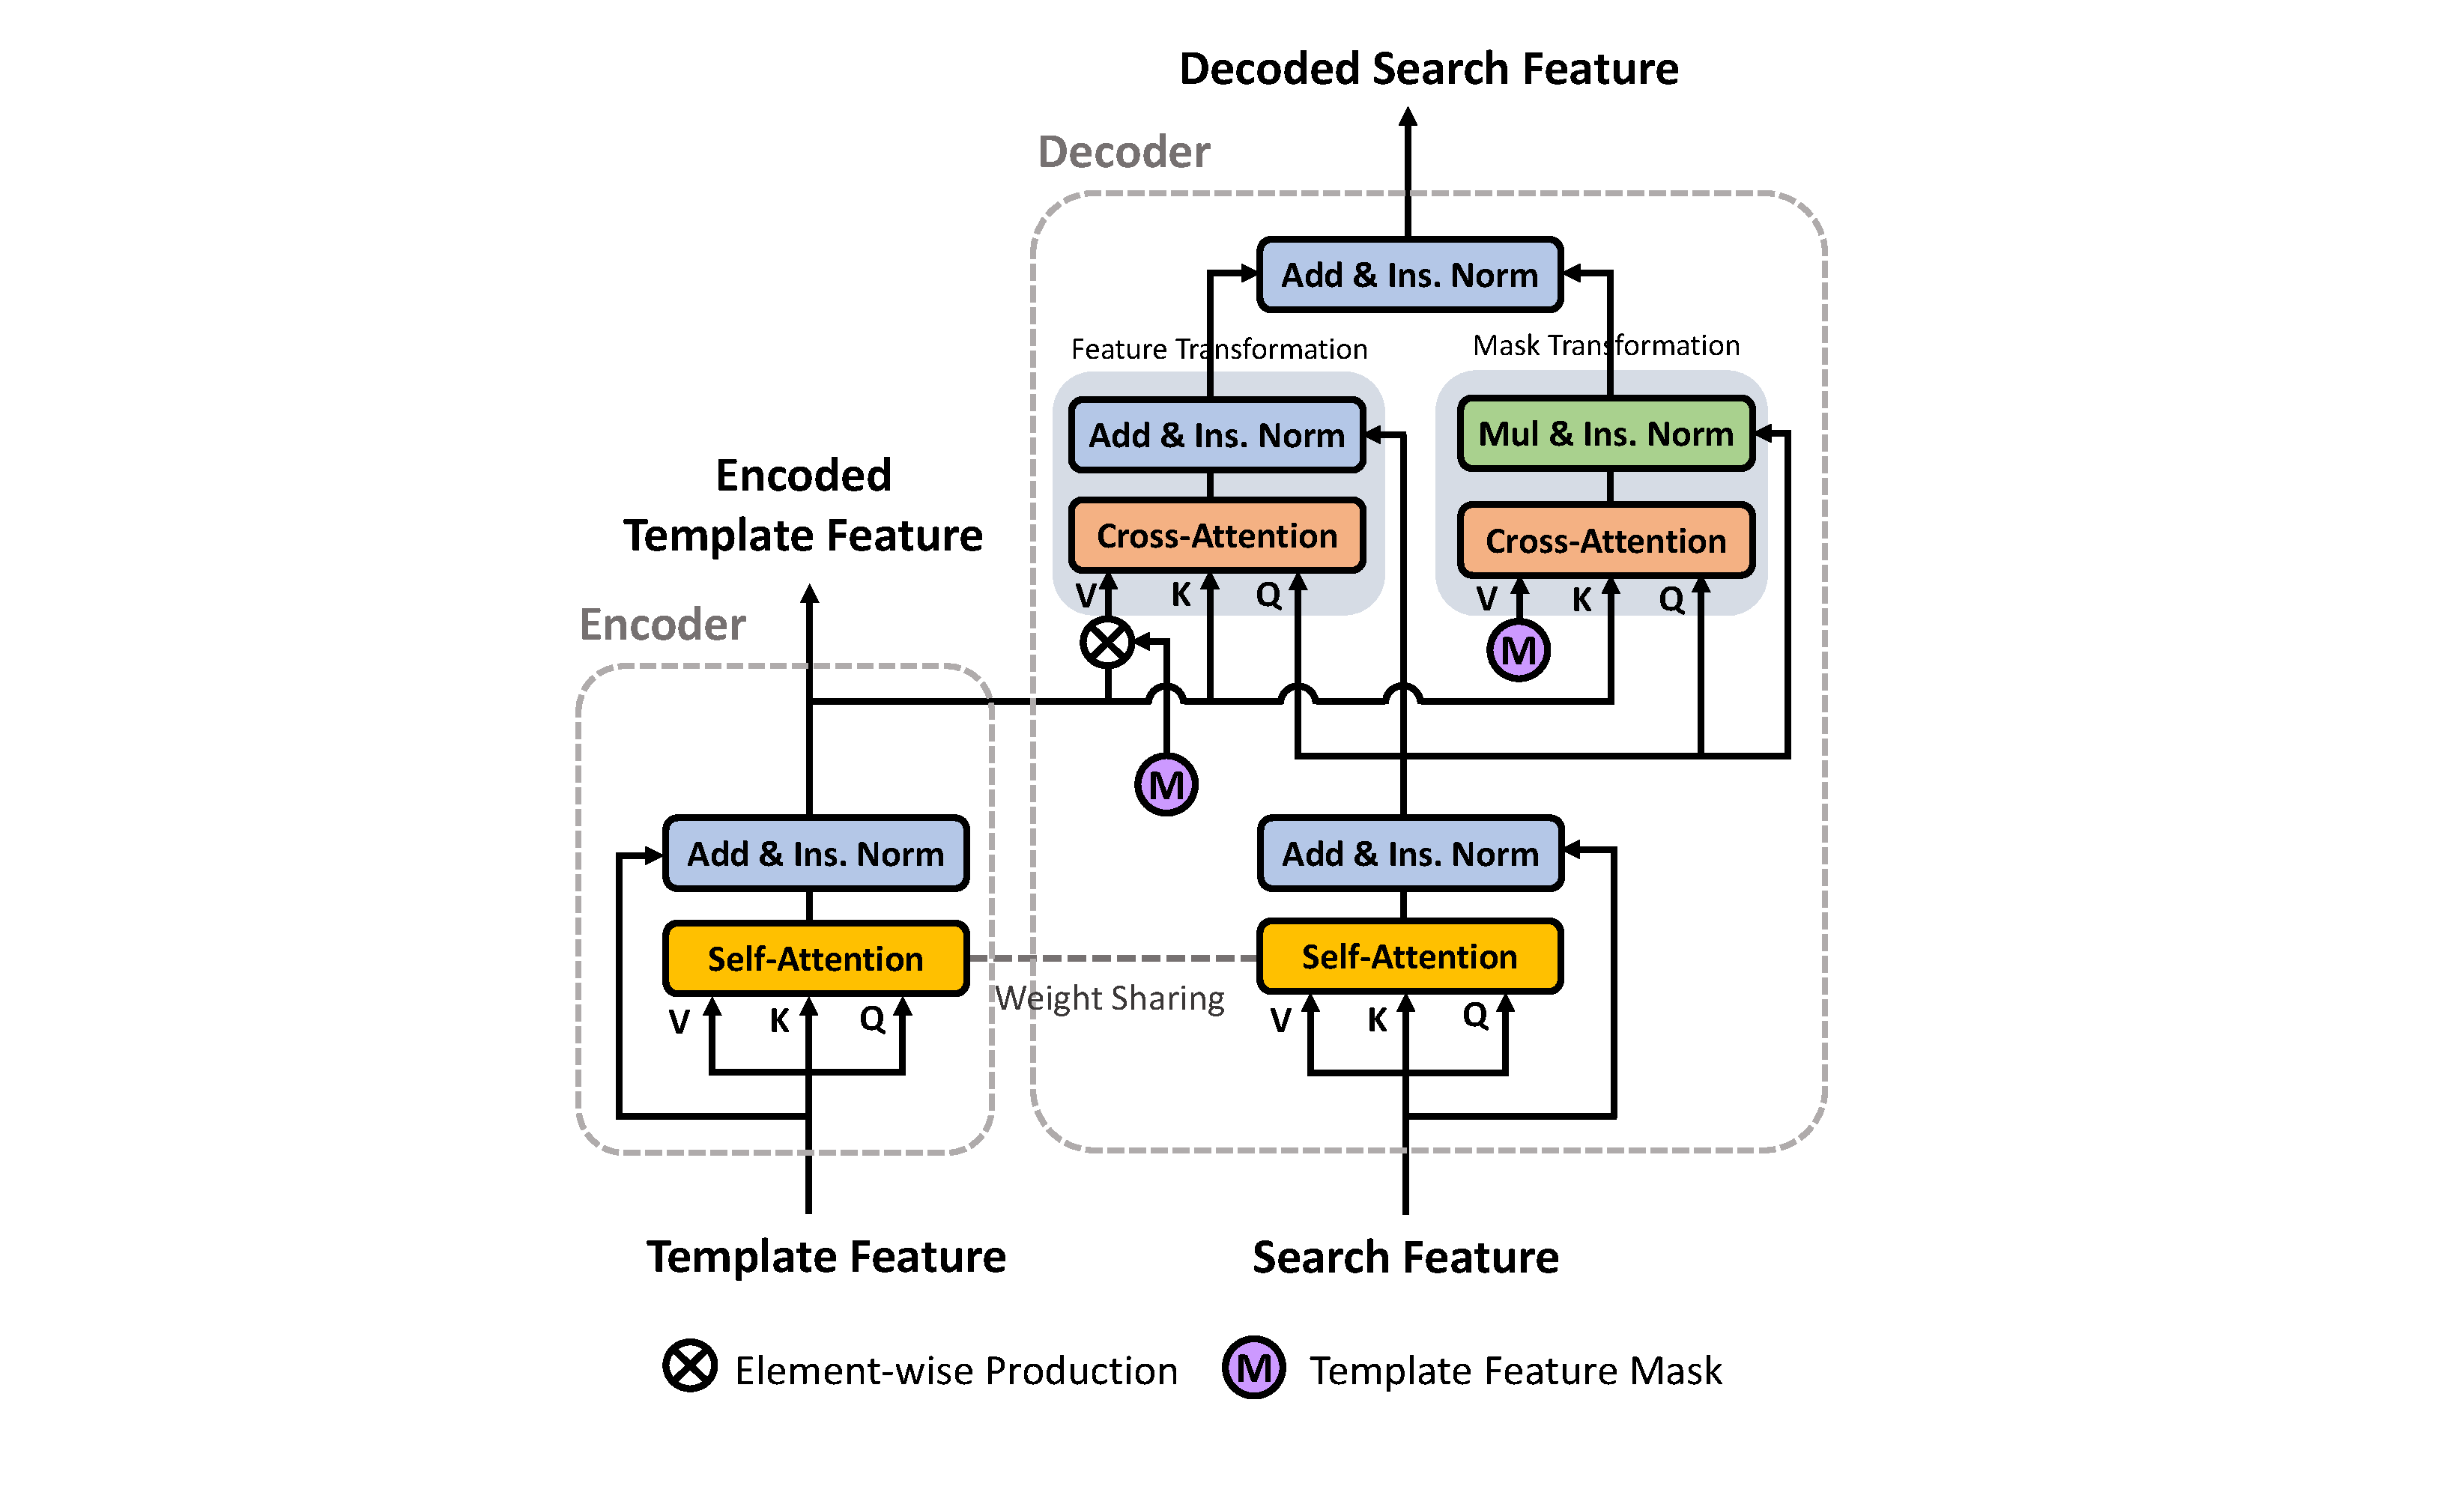
\includegraphics[width=4cm, height=3cm]{assets/main.pdf}}
	\caption{(a) The Proposed Siamese-like Pipeline, (b) The Encoder-Decoder Transformer used in the branches.}
	\label{fig:imgs}
\end{figure}

\section{Methods}
The proposed pipeline consists of two branches: The template branch and the search branch. The template branch takes multiple target templates and extracts features and corresponding masks used to detect the target in the later pipeline such as DCF~\cite{DiMP, ATOM} or Siamese~\cite{SiamFC}. In this branch, the transformer encoder captures the temporal relationships between each template and, thus, reinforces desirable features and suppresses noise across templates. On the other hand, the search branch generates decoded features that highlight the potential target areas using search frames and the features encoded by the template branch (Fig.~\ref{fig:imgs}).

\subsection{The Template Branch: Transformer Encoder}
At timestamp 0, the encoder transformer takes the concatenation of templates created by data augmentations. The encoder transformer has similar architecture to the original one~\cite{SA} (Fig.~\ref{fig:imgs}). After the first timestamp, search frames that show high accuracy are used as pseudo templates. The process models the temporal relationship. The transformed output feature has the same shape as the concatenated templated fed as the input. The pipeline propagates the transformed feature to the search branch's decoder transformer.

\subsection{The Search Branch: Transformer Decoder}
The decoder takes the search frame features and the extracted template features. The decoder first transforms the search features using the self-attention that is shared with the encoder. Then, the decoder inputs the transformed search features and the template features to cross-attention to generate decoded features. The cross-attention introduces cross-frame relationships to the decoded features.

\subsection{DCF or Siamese Pipeline}
Given the extracted template features and decoded response map, we generate predictions using the existing DCF~\cite{DiMP, ATOM} and Siamese ~\cite{SiamFC}, which basically convolving the decoded features using the template features and masks.

\subsection{Results}
The proposed method beats the existing state-of-the-art techniques with a comfortable margin. Furthermore, the provided qualitative results show that the proposed method refines the response maps. Finally, the ablation experiments show that the transformer helps to improve tracking performance.

\section{Personal Note}
The paper is challenging to understand because the description skips or omits some vital information such as inputs and outputs or the shape of ground truths. Moreover, I believe that section 3 is helpful to only those already familiar with this task. Nevertheless, the proposed method, which tries to capture the temporal information, seems compelling and insightful.


{\small
\bibliographystyle{ieee}
\bibliography{egbib}
}


\end{document}
